
\subsection{Selección del modelo definitivo para el proyecto}

% REVISAR, TAL VEZ B3 SEA MEJOR, HABRIA QUE HACER PRUEBAS
Con base en la comparación, se selecciona EfficientNet-B3 como el modelo definitivo para este proyecto. Esta arquitectura ofrece la mayor precisión en ImageNet entre los candidatos viables para móvil, con un tamaño de 48 MB que resulta perfectamente manejable para su despliegue mediante TFLite en Android.

%A diferencia de ResNet-50, su tamaño reducido lo hace apto para integrarse en la aplicación móvil sin comprometer el rendimiento del dispositivo. Frente a MobileNetV3, ofrece una precisión superior manteniendo un tamaño comparable. 

\begin{figure}[H]
    \centering
    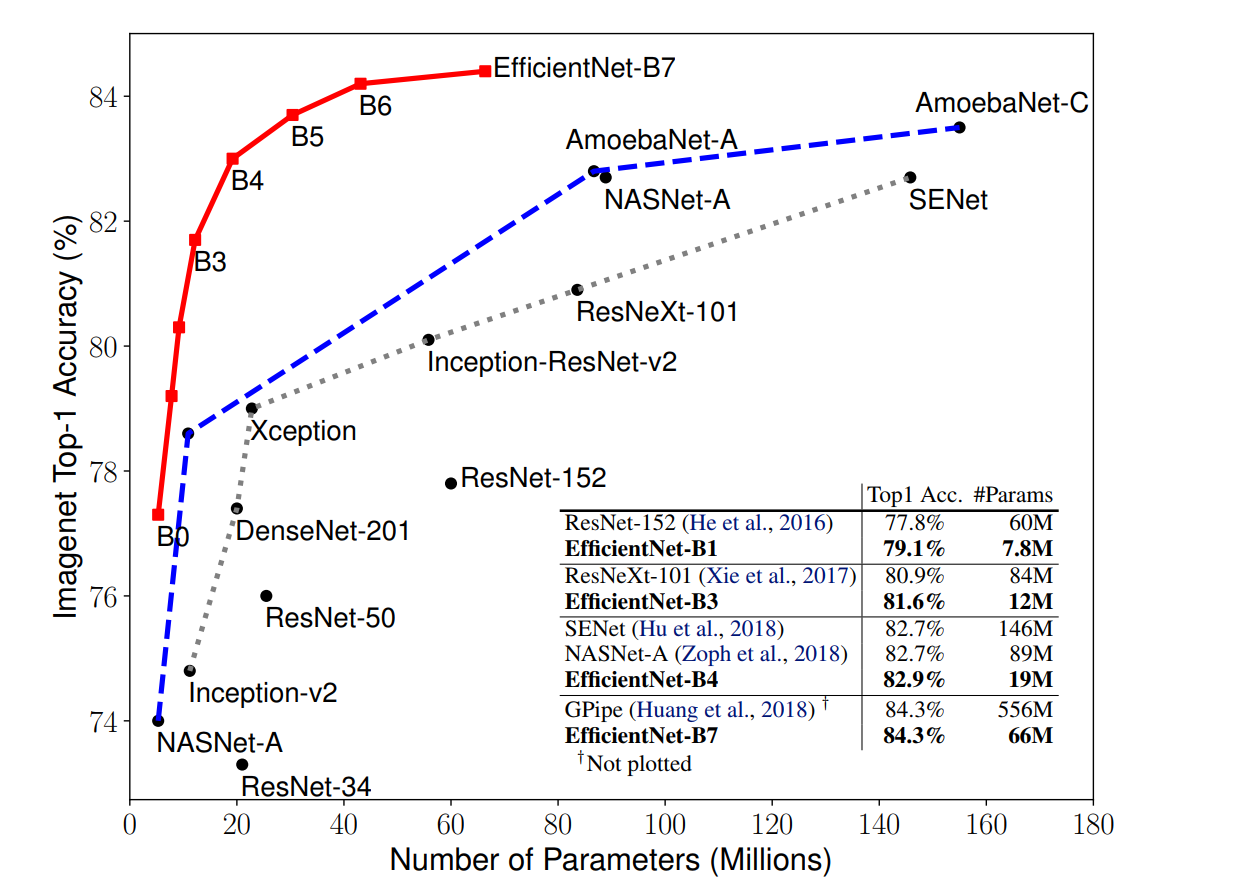
\includegraphics[width=0.6\textwidth]{images/C5/modelpower.png}
    \caption{Diagrama comparativo con diferentes arquitecturas de CNNs. Tomado de 
    \cite{Tan2019EfficientNetRM}}
    \label{fig:comparativaModelos}
\end{figure}

Adicionalmente, EfficientNet-B3 está disponible como modelo preentrenado en \texttt{tf.keras.apps}, lo que facilita su uso con la estrategia de transfer learning y fine-tuning descrita en la sección anterior.